\documentclass{article}
\usepackage[T1]{fontenc}
\usepackage{lmodern}
\usepackage{graphicx}
\usepackage{amsmath,amssymb}
\usepackage[a4paper,margin=2cm]{geometry}
\usepackage[absolute,overlay]{textpos}
\setlength{\TPHorizModule}{1mm}
\setlength{\TPVertModule}{1mm}
\usepackage[indonesian]{babel}
\usepackage{hyperref}
\setlength{\emergencystretch}{2em}
% unit: Halaman 51

\begin{document}

% === Halaman 51 (llm) ===

\section*{Kriptografi pada zaman Mesir Kuno}

\vspace{163.05mm}

\begin{itemize}
    \item Bangsa Mesir 4000 tahun yang lalu menggunakan \textit{hieroglyph} yang tidak standard untuk menulis pesan di dinding piramid.
\end{itemize}

\vspace{5mm}

% deskripsi: Foto prasasti dengan tulisan hieroglif Mesir Kuno yang dipahat pada permukaan batu.
% bbox normalisasi: [0.2330, 0.3930, 0.7310, 0.9420]
\begin{textblock*}{104.58mm}(48.93mm,116.72mm)
\noindent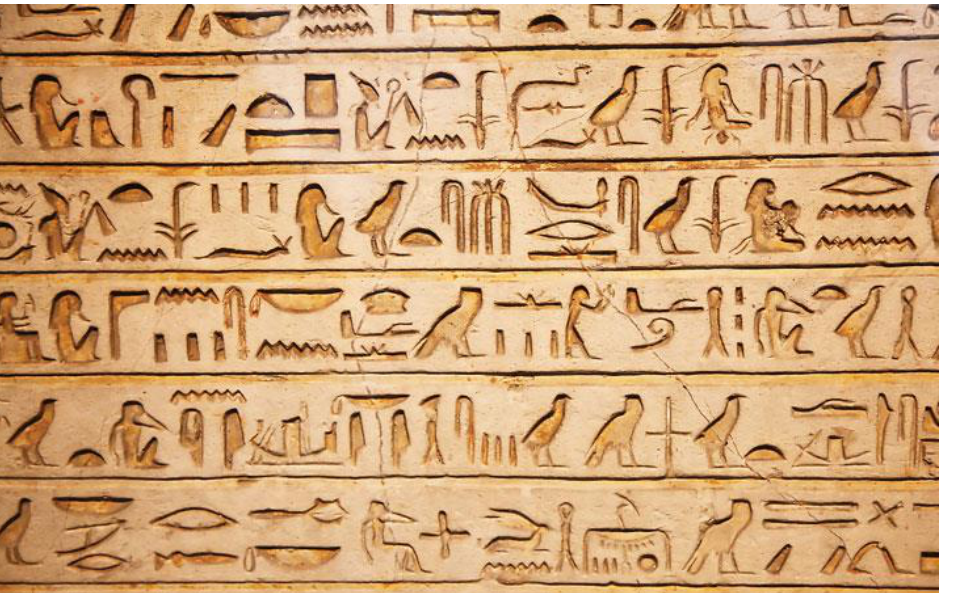
\includegraphics[width=104.58mm,height=163.05mm]{../../images/llm/page_051_img_01.png}%
\end{textblock*}

\end{document}
